\documentclass{beamer}

\usepackage[utf8]{inputenc}
\usepackage{forest}
\usepackage{tikz}
\usepackage{amsmath}
\usetikzlibrary{arrows,automata,positioning,backgrounds}



\usetheme{default}  %% Themenwahl
\beamertemplatenavigationsymbolsempty


\newcommand{\UC}[0]{uniquely decodable codes }
\newcommand{\IC}[0]{instantenous codes }

\title{Ungleichungen von Kraft \& McMillan}
\subtitle{Proseminar Informationstheorie}
\author{Phil Pützstück}
\date{\today}

\setbeamerfont{myTOC}{series=\bfseries,size=\Large}
\AtBeginSection[]{\frame{\frametitle{Inhalt}
\usebeamerfont{myTOC}\tableofcontents[current]}}

\begin{document}
\maketitle

\section{Bäume}
\begin{frame}
    \frametitle{Motivation / Überblick}
    \begin{itemize}
        \setlength\itemsep{1em}
        \item Gesehen, dass \UC und \IC sehr nützlich.
        \item Wann bzw. unter welchen Bedingungen existieren diese?
        \item Insbesondere: Wortlängen und Größe des Code-Alphabets
        \item Ungleichungen setzen diese Aspekte in Relation
    \end{itemize}
\end{frame}

\begin{frame}
    \frametitle{Bäume}
    \begin{columns}
    \begin{column}{0.5\textwidth}
        Baum $T = (V, E)$. Knotenmenge $V(T) := V$.
        Kantenmenge $E(T) := E$.\\

        \begin{itemize}
            \item ungerichtet
            \item azyklisch
            \item zusammenhängend
            \pause
            \item eindeutige Wurzel $root(T)$
            \pause
            \item Höhe $height(v), v \in V$
        \end{itemize}
        \pause
        Nenne $T$ $r$-är wenn jeder Knoten
        mit Ausnahme von Blättern
        genau $r \in \mathbb{N}$ Kinder hat.
    \end{column}

    \begin{column}{0.5\textwidth}
        \begin{center}
            \only<1,2,3>{\onslide\begin{tikzpicture}
                [scale=0.8, auto=left]
                \tikzset{edge/.style = {> = latex'}}
                \only<1>{\node[circle,draw] (q1) at (0,4)  {$a$};}
                \only<2->{\node[circle,draw,fill=red] (q1) at (0,4) {\textcolor{white}{$a$}};}
                \node[circle,draw] (q2) at (0,2)  {$b$};
                \node[circle,draw] (q3) at (2,2)  {$c$};
                \node[circle,draw] (q4) at (0,0)  {$d$};
                \node[circle,draw] (q5) at (2,0)  {$e$};
                \node[circle,draw] (q6) at (4,0)  {$f$};

                \foreach \from/\to in {q1/q2,q1/q3,q2/q4,q3/q5,q3/q6}
                    \draw[edge] (\from) to (\to);

                \only<3>{
                    \draw (q1) [->,red,line width=1pt] -- node[left] {1} (q2);
                    \draw (q2) [->,red,line width=1pt] -- node[left] {2} (q4);
                    \node [below = 0.1 cm of q4] {\small{$height(d) = 2$}};
                }
            \end{tikzpicture}
            }
            \only<4>{\onslide
                \centerline{2-är bzw. binär}\

                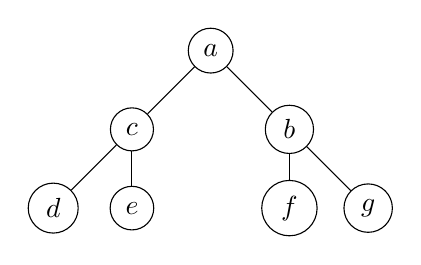
\begin{tikzpicture}
                    [scale=1, auto=left]
                    \tikzset{edge/.style = {> = latex'}}
                    \node[circle,draw] (q1) at (0,0)    {$a$};
                    \node[circle,draw] (q2) at (1,-1)   {$b$};
                    \node[circle,draw] (q3) at (-1,-1)  {$c$};
                    \node[circle,draw] (q4) at (-2,-2)  {$d$};
                    \node[circle,draw] (q5) at (-1,-2)  {$e$};
                    \node[circle,draw] (q6) at (1,-2)   {$f$};
                    \node[circle,draw] (q7) at (2,-2)   {$g$};

                    \foreach \from/\to in {q1/q2,q1/q3,q2/q6,q2/q7,q3/q4,q3/q5}
                        \draw[edge] (\from) to (\to);
                \end{tikzpicture}
            }
         \end{center}
    \end{column}
    \end{columns}
\end{frame}

\begin{frame}[t]
    \frametitle{Teilbäume und Ordnung von Knoten}
    \only<1-2>{
        $T,T'$ gewurzelte Bäume.
        \begin{itemize}
            \item Schreibe $T'\leq T$ wenn $T'$ Teilgraph von $T$.
            \pause
            \item Schreibe $T' \leq_{\color{red}{r}} T$ wenn $T' \leq T$ und $T,T'$ {\color{red}$r$-är}.\\[5pt]
        \end{itemize}
    }
    \only<3>{Für $v,v' \in T$ schreiben wir $v' \leq v$, genau dann, wenn der eindeutige Pfad von $root(T)$ zu $v$
    den Knoten $v'$ besucht.\\
    Hier $root(T) = a$}
    \pause
    \begin{center}
        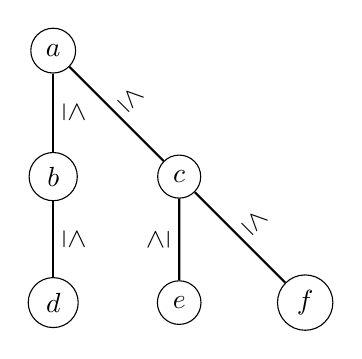
\begin{tikzpicture}
            [scale=0.8, auto=left]
            \tikzset{edge/.style = {> = latex'}}
            \node[circle,draw] (q1) at (0,4)  {$a$};
            \node[circle,draw] (q2) at (0,2)  {$b$};
            \node[circle,draw] (q3) at (2,2)  {$c$};
            \node[circle,draw] (q4) at (0,0)  {$d$};
            \node[circle,draw] (q5) at (2,0)  {$e$};
            \node[circle,draw] (q6) at (4,0)  {$f$};

        \only<3>{
            \draw (q1) [-,line width=.8pt] -- node[sloped,above] {$\leq$} (q2);
            \draw (q1) [-,line width=.8pt] -- node[sloped,above] {$\leq$} (q3);
            \draw (q2) [-,line width=.8pt] -- node[sloped,above] {$\leq$} (q4);
            \draw (q3) [-,line width=.8pt] -- node[sloped,above] {$\geq$} (q5);
            \draw (q3) [-,line width=.8pt] -- node[sloped,above] {$\leq$} (q6);
        }
        \end{tikzpicture}
    \end{center}
\end{frame}

\begin{frame}[t]
    \frametitle{Teilbäume und Ordnung von Knoten}
    Sei $v \in V(T)$. Wir wollen $v$ und seine ''Nachfolger'' $w \in V(T), v \leq w$ von $T$ inklusive
    Kanten ''ausschneiden''.

    \begin{center}
        \begin{tikzpicture}
            [scale=0.8, auto=left]
            \tikzset{edge/.style = {> = latex'}}

            \node[circle,draw] (q1) at (0,4)  {$a$};
            \node[circle,draw] (q2) at (0,2)  {$b$};
            \node[circle,draw] (q4) at (0,0)  {$d$};

            \draw (q1) [-,line width=.8pt] -- (q2);
            \draw (q2) [-,line width=.8pt] -- (q4);

            \only<1>{
                \node[circle,draw] (q5) at (2,0)  {$e$};
                \node[circle,draw] (q6) at (4,0)  {$f$};

                \draw (q3) [-,line width=.8pt] -- (q5);
                \draw (q3) [-,line width=.8pt] -- (q6);
            }

            \only<1-2>{
                \draw (q1) [-,line width=.8pt] -- (q3);
            }

            \only<1-3>{
                \node[circle,draw,fill=red] (q3) at (2,2)  {\textcolor{white}{$v$}};
            }

            \only<2-3>{
                \node[circle,draw,fill=red] (q5) at (2,0)  {\textcolor{white}{$w$}};
                \node[circle,draw,fill=red] (q6) at (4,0)  {\textcolor{white}{$w$}};

                \draw (q3) [-,line width=.8pt,color=red] -- node[sloped,above] {$\geq$} (q5);
                \draw (q3) [-,line width=.8pt,color=red] -- node[sloped,above] {$\leq$} (q6);
            }

            \only<3>{
                \node at (-1.6, 4) {$root(T) = $};
                \node at (3.8, 2) {$ = root(T')$};
                \draw (q1) [dashed,line width=.5pt] -- (q3);
            }

            \only<4>{
                \node at (-2,4) {$root(T \setminus v) = $};
                \node at (3,4) {};
            }
        \end{tikzpicture}
    \end{center}

    \only<3->{
        Definiere $T \setminus v := T \setminus T'$, wobei $T' \leq T$ der Teilbaum
        von $T$ mit Wurzel $v \in V(T) \setminus \{root(T)\}$ ist.\\
        Insbesondere ist $T \setminus v$ wieder ein gewurzelter Baum.
    }
\end{frame}

\begin{frame}
    \frametitle{Code als Baum}
    Sei $\mathcal{C}$ ein Code über dem Code-Alphabet $\{0,1,2\}$.\\
    $\mathcal{C}$ als Teilmenge von $V(T)$, wobei $T$:
    \begin{center}
        \begin{forest}
            [$\varepsilon$
                [$0$
                    [$00$],
                    [$01$],
                    [$02$]
                ],
                [$1$
                    [$10$],
                    [$11$],
                    [$12$]
                ],
                [$2$
                    [$20$],
                    [$21$],
                    [$22$]
                ]
            ],
        \end{forest}\\
        \centerline{\LARGE{\dots}}
    \end{center}
    \pause
\end{frame}

\section{Ungleichung von Kraft}
\begin{frame}
    \frametitle{Ungleichung von Kraft}
    Seien $q,r \in \mathbb{N}, l \in \mathbb{N}^q$. Dann existiert ein $r$-ärer instantaneous Code $\mathcal{C}$
    mit Wortlängen $l$ genau dann, wenn
    $$
        \sum_{k=1}^{q} \frac{1}{r^{l_k}} \leq 1
    $$\\[20pt]
    \pause

    Annahmen:

    \begin{itemize}
        \item Anzahl Code-Wörter $q > 1$
        \pause
        \item Wortlängen $l$ aufsteigend sortiert und $l_1 > 0$
        \pause
        \item Code-Alphabet von $\mathcal{C}$ ist $[0,r-1]$
    \end{itemize}
\end{frame}

\begin{frame}
    \frametitle{Ungleichung von Kraft: ''$\,\Longrightarrow\,$''}
    Richtung ''$\sum_{k=1}^{q} \frac{1}{r^{l_k}} \leq 1 \,\Longrightarrow\,$ $\mathcal{C}$ existiert''.\\[10pt]
    \pause
    Nach [JJ00] sind die instantaneous Codes genau die Präfixcodes.\\[10pt]
    \pause
    Konstuiere Codewörter $w_i$ mit $|w_i| = l_i$ via endlicher Induktion über $i$.
    Betrachte dabei den zum Code-Alphabet zug. Baum und wähle die $w_i$ so, dass
    am Ende $\mathcal{C} = \{w_i \mid i \in [1,q]\}$ ein Präfixcode ist.
\end{frame}

\begin{frame}
    \frametitle{Ungleichung von Kraft: ''$\,\Longrightarrow\,$''}

    \begin{columns}
    \begin{column}{0.5\textwidth}
        \only<1-3>{Sei also $i = 1$. Wähle Knoten $v_w$ der Höhe $l_1 > 0$ beliebig und setze $w_1 := w$.\\[10pt]\pause
        Setze $h = l_q$ (max. Wortlänge) und $\mathcal{T}_1 := \mathcal{T}_r^h \setminus v_{w_1}$.\\[10pt]}\pause
        $\mathcal{T}_1$ hat dann noch
        $r^h - r^{h -l_1}$ Blätter.\\
        \only<4->{
            Weiter gilt:
            $$
                r^h - r^{h - l_1} = r^h\left(1 - \sum_{k=1}^{1} \frac{1}{r^{l_k}}\right)
            $$
            \only<5->{
                $$
                    > r^h\left(1 - \sum_{k=1}^{q} \frac{1}{r^{l_k}}\right) \only<6>{\geq 0}
                $$
            }
        }
    \end{column}

    \begin{column}{0.5\textwidth}
        \onslide\begin{center}
            \only<1>{
            \begin{forest}
                [$v_\varepsilon$
                    [$v_0$
                        [\dots]
                        [\dots]
                    ]
                    [$v_1$
                        [\dots
                            [$v_w$,color=red,
                                [$v_{w0}$
                                    [\dots],
                                    [\dots]
                                ],
                                [$v_{w1}$
                                    [\dots],
                                    [\dots]
                                ]
                            ],
                            [,phantom]
                        ]
                        [\dots]
                    ]
                ]
            \end{forest}
            }
            \only<2>{
            \begin{forest}
                [$v_\varepsilon$
                    [$v_0$
                        [\dots]
                        [\dots]
                    ]
                    [$v_1$
                        [\dots
                            [$v_w$,color=red, tikz={\node [draw,red,fit=()(!1)(!11)(!2)(!22)] {};}
                                [$v_{w0}$
                                    [\dots],
                                    [\dots]
                                ],
                                [$v_{w1}$
                                    [\dots],
                                    [\dots]
                                ]
                            ],
                            [,phantom]
                        ]
                        [\dots]
                    ]
                ]
            \end{forest}
            }
            \only<3->{
                \begin{tikzpicture}
                    \node[color=red] at (0.5,-3) {$v_{w_1}$};
                    \node at (0,-1.5) {$\mathcal{T}_1$};

                    \draw (0,0) node[above]{$v_\varepsilon$}
                        -- (-2.5,-4)
                        -- (-.5,-4)
                        -- (0.5,-2.4)
                        -- (1.5,-4)
                        -- (2.5,-4)
                        -- cycle;

                    \draw[|-|] (-.5,-4.5) -- node[below] {$r^{h-l_1}$} (1.5,-4.5);

                    \draw[|-|] (-2.5,-5.4) -- node[below] {$r^h$} (2.5,-5.4);
                \end{tikzpicture}
            }
        \end{center}
    \end{column}
    \end{columns}
\end{frame}

\begin{frame}
    \frametitle{Ungleichung von Kraft: ''$\,\Longrightarrow\,$''}
    Sei nun $i \in [1,q-1]$ sodass $\mathcal{C} = \{w_j \mid j \in [1,i]\}$ ein Präfix-Code
    mit $|w_j| = l_j$ ist, und $\mathcal{T}_i$ noch mindestens 1 Blatt $v_x$ hat.\\[10pt]\pause

    \begin{columns}
    \begin{column}{0.77\textwidth}
        \begin{itemize}
            \item $\mathcal{T}_i$ zusammenhängend\\[10pt]
            \item also ex. $v_w \in V(\mathcal{T}_i)$ mit $height(v_w) = l_{i+1} \leq h$\\[10pt]
            \item Setze $w_{i+1} := w$.
        \end{itemize}
    \end{column}
    \begin{column}{0.23\textwidth}\onslide
        \begin{center}
            \only<1>{
                \begin{forest}
                    [$v_\varepsilon$
                        [\vdots
                            [$v_{x}$]
                        ]
                    ]
                \end{forest}
            }
            \only<2->{
                \begin{forest}
                    [$v_\varepsilon$
                        [\vdots
                            [$v_{w_{i+1}}$,color=blue
                                [\vdots
                                    [$v_x$]
                                ]
                            ]
                        ]
                    ]
                \end{forest}
            }
        \end{center}
    \end{column}
    \end{columns}
\end{frame}

\begin{frame}[t]
    \frametitle{Ungleichung von Kraft: ''$\,\Longrightarrow\,$''}
    \only<1>{Sei $j \in [1,i]$. Wir haben bereits alle Knoten $v_w \geq v_{w_j}$ im Schritt
    $\mathcal{T}_j := \mathcal{T}_{j-1} \setminus v_{w_j}$ gelöscht. Da wir $v_{w_{i+1}}$
    aus $\mathcal{T}_i$ gewählt haben, kann also \textbf{nicht} $v_{w_j} \leq v_{w_{i+1}}$ gelten.} \pause
    \only<2->{
        Folglich haben wir auch $w_j \not\sqsubseteq w_{i+1}$ für $j \in [1,i]$. $\mathcal{C}$ bleibt also
        durch Wahl von $w_{i+1}$ ein Präfix-Code ($l_j \leq l_{i+1}$, also $w_{i+1} \not\sqsubseteq w_j$).
    }
    \pause
    \only<3->{
        \\[10pt]
        Wenn nun $i+1 = q$ war, so sind wir fertig, da wir das letzte Wort $w_q$ soeben $\mathcal{C}$
        hinzugefügt haben.\pause\\[10pt]
        Falls hingegen $i+1 < q$, so definiere $\mathcal{T}_{i+1} := \mathcal{T}_i \setminus v_{w_{i+1}}$.\\
        Dann hat $\mathcal{T}_{i+1}$ immernoch mindestens 1 Blatt, denn:
        \only<4>{
        $$
            \mathcal{T}_i\ \text{hat nach Konstruktion}\quad
            r^h - \sum_{k=1}^{i} r^{h-l_k}
            \quad\text{Blätter}
        $$
        }
        \pause
        \only<5->{
            \\
            $\mathcal{T}_{i+1}$ hat nach Konstruktion also:
            $$
                r^h - \sum_{k=1}^{i+1} r^{h-l_k}
                \pause
                > r^h - \sum_{k=1}^{q} r^{h-l_k}
                \pause
                = r^h \left(1 - \sum_{k=1}^{q} \frac{1}{r^{l_k}}\right)
                \pause
                \geq 0
            $$
            Blätter. Somit können wir einen Präfix-Code $\mathcal{C}$ unter den gegebenen Bedingungen konstruieren.
            Dieser ist nach [JJ00] auch instantaneous.
        }
    }

    \only<1-2>{
    \begin{center}\onslide
        \begin{tikzpicture}
            \node[color=red] at (2,-4) {$v_{w_1}$};
            \node[color=red] at (-4.5,-5) {$v_{w_j}$};
            \node[color=red] at (-2.5,-5.2) {$v_{w_k}$};
            \node[color=blue] at (-0.2,-5) {$v_{w_{i+1}}$};
            \node at (-1,-5.8) {$v_x$};
            \node at (0,-1.5) {$\mathcal{T}_i$};

            \draw (0,0)
                -- (-4.5,-4.5)
                -- (-3.5,-5.5)
                -- (-3.25,-5.5)
                -- (-2.5,-4.75)
                -- (-1.75,-5.5)
                -- (0,-5.5)
                -- (2,-3.5)
                -- (4,-5.5)
                -- (5.5,-5.5)
                -- cycle;

            \draw[dashed] (0,0)
                -- (0,-0.15)
                -- (-1,-1.15)
                -- (0,-2)
                -- (-1.5,-3.5)
                -- (-1,-4)
                -- (-1.25,-4.25)
                -- (-0.5,-5)
                -- (-1,-5.5);
        \end{tikzpicture}
    \end{center}
    }
\end{frame}

\begin{frame}[t]
    \frametitle{Ungleichung von Kraft: ''$\,\Longleftarrow\,$''}
    \only<1-2>{
        Nun zeigen wir, dass wenn $\mathcal{C}$ instantaneous, also ein Präfix-Code ist, auch
        die Ungleichung gelten muss. \pause\\
        Betrachte für $i \in [1,q]$ die Menge der Blätter unter $v_{w_i}$:
    }
    \only<2->{
        $$
            {\color{red}L_i} := \{v \in V(\mathcal{T}_r^h) \mid v_{w_i} \leq v \land height(v) = h\}
        $$
        \begin{center}\onslide
            \begin{tikzpicture}
                \node at (0,-1) {$\mathcal{T}_r^h$};
                \node at (.5, -2.3) {$v_{w_i}$};
                \node[color=red] at (.5, -4.3) {$L_i$};

                \draw (0,0)
                    -- (-4,-4)
                    -- (4,-4)
                    -- cycle;

                \draw[dashed] (-1,-4) -- (.5, -2.5) -- (2,-4);

                \draw[line width = 2pt, color=red] (-1,-4) -- (2,-4);
            \end{tikzpicture}
        \end{center}
    }
\end{frame}

\begin{frame}[t]
    \frametitle{Ungleichung von Kraft: ''$\,\Longleftarrow\,$''}
    Wir wissen nun, dass für $i,j$ mit $i \neq j$ auch $L_i \cap L_j = \varnothing$ gelten muss\pause
    \only<2-5>{
        \\[10pt]
        Sei o.E. $i < j, v_w \in L_i \cap L_j$, also $v_w$ gleichzeitig Blatt unter $v_{w_i}$ und $v_{w_j}$.
        \pause
        Dann gilt:
        $$
            v_{w_i} \leq v_w \land v_{w_j} \leq v_w
            \pause \,\Longrightarrow\,
            w_i \sqsubseteq w \land w_j \sqsubseteq w
            \pause \,\Longrightarrow\,
            w_i \sqsubseteq w_j
        $$
        Widerpruch, denn $w_i, w_j \in \mathcal{C}$ und $\mathcal{C}$ ist Präfix-Code!
        \pause
    }
    \only<6->{
        \\[10pt]
        Wir wissen weiter, dass $\mathcal{T}_r^h$ nur $r^h$ Blätter hat, und $|L_i| = r^{h-l_i}$.
        \only<7->{
            \\[10pt]
            Damit haben wir nun:
            $$
                r^h \geq \left| \bigcup_{i \in [1,q]} L_i \right|
            \only<8->{
                = \sum_{i=1}^{q} |L_i|
            }\only<9->{
                = \sum_{i=1}^{q} r^{h-l_i}
                = r^h\sum_{i=1}^{q} \frac{1}{r^{l_i}}
            }
            $$
            \only<11->{
                $$
                    \,\Longleftrightarrow\, \sum_{i=1}^{q} \frac{1}{r^{l_i}} \leq 1
                $$
                Dies war zu zeigen. \hfill $\square$
            }
        }
        \only<6>{
            \begin{center}\onslide
                \begin{tikzpicture}
                    \node at (0,-1) {$\mathcal{T}_r^h$};
                    \node at (.5, -2.3) {$v_{w_i}$};
                    \node[color=red] at (.5, -4.3) {$L_i$};

                    \draw (0,0)
                        -- (-4,-4)
                        -- (4,-4)
                        -- cycle;

                    \draw[dashed] (-1,-4) -- (.5, -2.5) -- (2,-4);

                    \draw[line width = 2pt, color=red] (-1,-4) -- (2,-4);

                    \draw[|-|] (-1,-4.6) -- node[below] {$r^{h-l_i}$} (2,-4.6);
                    \draw[|-|] (-4,-5.4) -- node[below] {$r^h$} (4,-5.4);
                    \draw[|-|] (-4.5,-4) -- node[left] {$h$} (-4.5, 0);
                    \draw[|-|] (4.5,-4) -- node[right] {$h-l_i$} (4.5, -2.5);
                    \draw[dotted, line width = 1pt] (4.5, -2.5) -- (.5, -2.5);
                \end{tikzpicture}
            \end{center}
        }
    }
\end{frame}

\begin{frame}
    \frametitle{Review of Kraft or smth.}

    Wir haben also gezeigt [...]

    \begin{itemize}
        \item Nach [JJ00] bekannt, dass instantaneous $\,\Longrightarrow\,$ uniquely decodable
        \item Jedoch vorraussetzungen für letzteres \textbf{nicht} schwächer:
    \end{itemize}

\end{frame}

\section{Ungleichung von McMillan}

\begin{frame}
    \frametitle{Ungleichung von McMillan}
    Seien $q,r \in \mathbb{N}, l \in \mathbb{N}^q$. Dann existiert ein $r$-ärer uniquely decodable Code $\mathcal{C}$
    mit Wortlängen $l$ genau dann, wenn
    \begin{equation}
        \sum_{k=1}^{q} \frac{1}{r^{l_k}} \leq 1
    \end{equation}\\[20pt]
    \pause

    Richtung ''$(1) \,\Longrightarrow\, \mathcal{C}$ existiert'' mit Kraft geschenkt.\\
\end{frame}

\end{document}
